\subsection{Entropi}

Entropi beskriver mængden af ''uorden'' i et billede. \\

Hvis alle pixels i et billede har samme værdi er entropien nul. Hvis billedet er perfekt ''histogram equalized'' er entropien højest. Når et billedes entropi nedsættes, mindskes mængden af information i billedet. Mængden af information kan siges at være lav, hvis den kan ''kommunikeres'' med en kort besked.\\

Ved høj entropi ændrer pixels sig ''unexpected'' og der skal af den grund større beskeder til at sende informationen.

Figur~\ref{fig:entropy} viser to billeder. Et med høj entropi og et med lav entropi (ikke nul).

\begin{figure}[H]
	\centering
	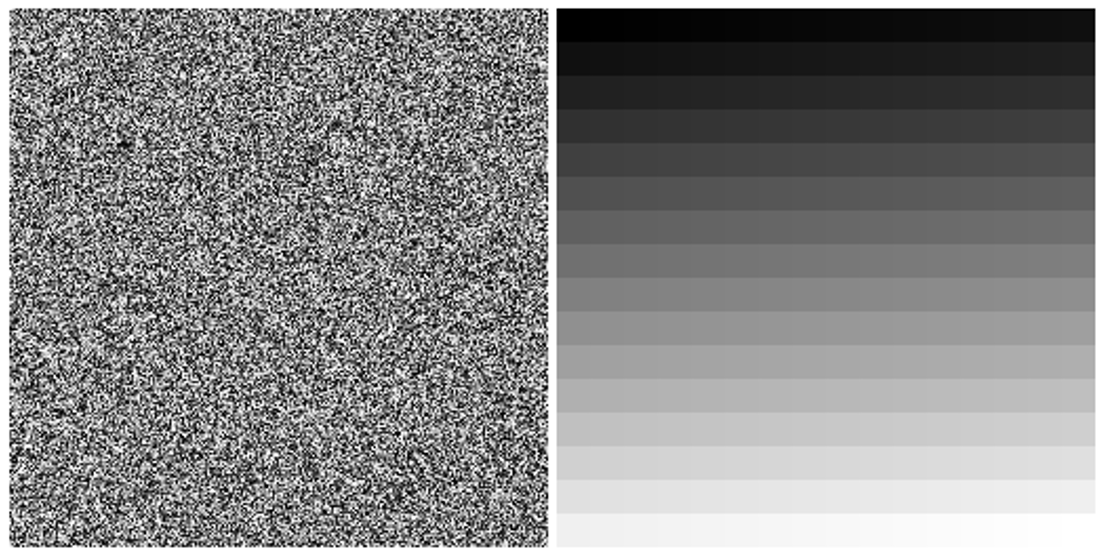
\includegraphics[width=0.7\linewidth]{figs/spm08/entropy}
	\caption{Venstre: høj entropi, højre: lav entropi.}
	\label{fig:entropy}
\end{figure}

Med Ligning~\ref{eq:entropy-image}  kan entropien i et billede beregnes. Her er $\widetilde{H}$ entropien, $L$ er intervalle og $p_r$ er en sandsynlighed for at en intensitet $r_k$ optræder.

\begin{equation}\label{eq:entropy-image}
\widetilde{H} =  - \sum_{k = 0}^{L-1} \; p_r (r_k) \; log_2 \; \; p_r (r_k)
\end{equation}